\section{Visión General de la Metodología}
La metodología propuesta se fundamenta en un esquema de control de bucle cerrado donde un agente inteligente interactúa constantemente con un entorno de tráfico simulado. Este sistema integra tres componentes principales:

\begin{enumerate}
    \item \textbf{Entorno de Simulación Microscópica:} Siguiendo el esquema experimental reportado en benchmarks y estudios de caso recientes, el entrenamiento y la evaluación se desarrollan sobre un simulador que permite observar y controlar el tráfico paso a paso \cite{benchmark_ault2021,case_gokulan2020}. En esta tesis, dicha plataforma se implementa en SUMO.
    \item \textbf{Agente de Control (DRL):} Implementado mediante \textbf{Proximal Policy Optimization (PPO)}, este agente toma decisiones de control semafórico basándose en el estado actual del cruce \cite{ppo_karedla2025,haps_ppo2025}.
    \item \textbf{Interfaz de Comunicación (TraCI):} Traffic Control Interface sirve como puente bidireccional, permitiendo al agente recibir observaciones del simulador y enviar comandos de control en tiempo real.
\end{enumerate}

El flujo de trabajo sigue el ciclo estándar de Aprendizaje por Refuerzo: en cada paso de tiempo $t$, el agente observa el estado $s_t$ del tráfico, selecciona una acción $a_t$ y recibe una recompensa $r_t$ que refleja la eficiencia de su decisión. Este proceso iterativo permite al agente optimizar su política de control $\pi_\theta$ para maximizar el desempeño a largo plazo.

\textbf{Detalle de Interacción:}
La sincronización entre el simulador y el agente es crítica. En cada paso de simulación $\Delta t$, TraCI detiene la ejecución de SUMO para extraer las variables de estado de los sensores inductivos simulados. Estos datos son procesados y normalizados antes de ser alimentados a la red neuronal del agente PPO. La red emite una distribución de probabilidad sobre las acciones posibles, de la cual se muestrea la siguiente fase semafórica. Finalmente, TraCI envía el comando al controlador del semáforo en SUMO y avanza la simulación al siguiente paso.

\begin{figure}[H]
    \centering
    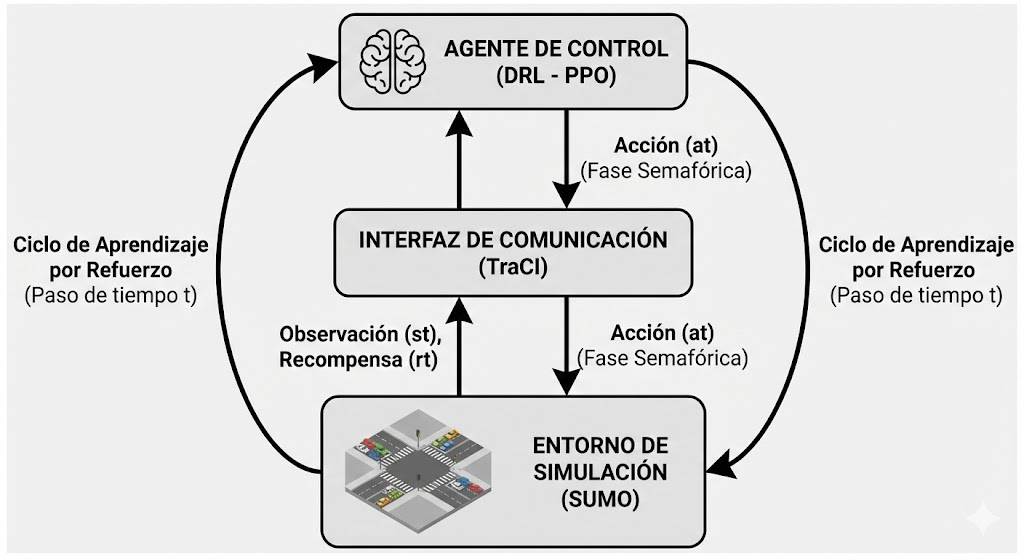
\includegraphics[width=0.8\textwidth]{images/grafico_overview.png}
    \caption{Arquitectura de control en bucle cerrado integrando SUMO, TraCI y el Agente PPO.}
    \label{fig:overview}
\end{figure}

\section{Diseño del cruce estudiado}
El escenario experimental consiste en una intersección aislada de cuatro aproximaciones (Norte, Sur, Este, Oeste), diseñada para replicar las condiciones de una arteria urbana principal.

\begin{itemize}
    \item \textbf{Geometría:} Cada aproximación cuenta con 3 carriles de 3.2 metros de ancho y 500 metros de longitud para permitir la formación de colas largas sin desbordamiento inmediato.
    \item \textbf{Fases Semafóricas:} En este estudio, una ``fase'' se define como el estado de señalización activo para todos los semáforos del cruce simultáneamente. Se definieron dos fases verdes principales:
    \begin{enumerate}
        \item \textbf{Fase NS (Fase 0):} Verde exclusivo para flujos Norte-Sur (duración variable).
        \item \textbf{Fase EO (Fase 2):} Verde exclusivo para flujos Este-Oeste (duración variable).
    \end{enumerate}
    Entre cambios de fase, se insertan fases de transición (amarillo: 3s, todo rojo: 2s) para garantizar la seguridad.
    \item \textbf{Sensores:} Se implementaron detectores de inducción simulados (E2) en cada carril para capturar variables de estado como ocupación y velocidad media en tiempo real.
\end{itemize}

\section{Modelado y configuración de SUMO}
Para someter al agente a condiciones de estrés realistas, se diseñó un perfil de tráfico dinámico de 60 minutos (3600 segundos) que simula la evolución de la demanda durante una hora pico. Este perfil se divide en cinco etapas críticas:

\begin{enumerate}
    \item \textbf{Calentamiento (0-900s):} Flujo bajo y balanceado para inicializar la red.
    \item \textbf{Pico Sur (900-1800s):} Incremento agresivo de la demanda en la dirección Sur-Norte, simulando el ingreso a la ciudad.
    \item \textbf{Transición (1800-2400s):} Retorno gradual a condiciones medias.
    \item \textbf{Pico Este (2400-3300s):} Alta demanda en la dirección transversal (Este-Oeste).
    \item \textbf{Ráfagas (3300-3600s):} Inyecciones aleatorias de alta densidad para evaluar la capacidad de recuperación rápida del agente.
\end{enumerate}

\begin{figure}[H]
    \centering
    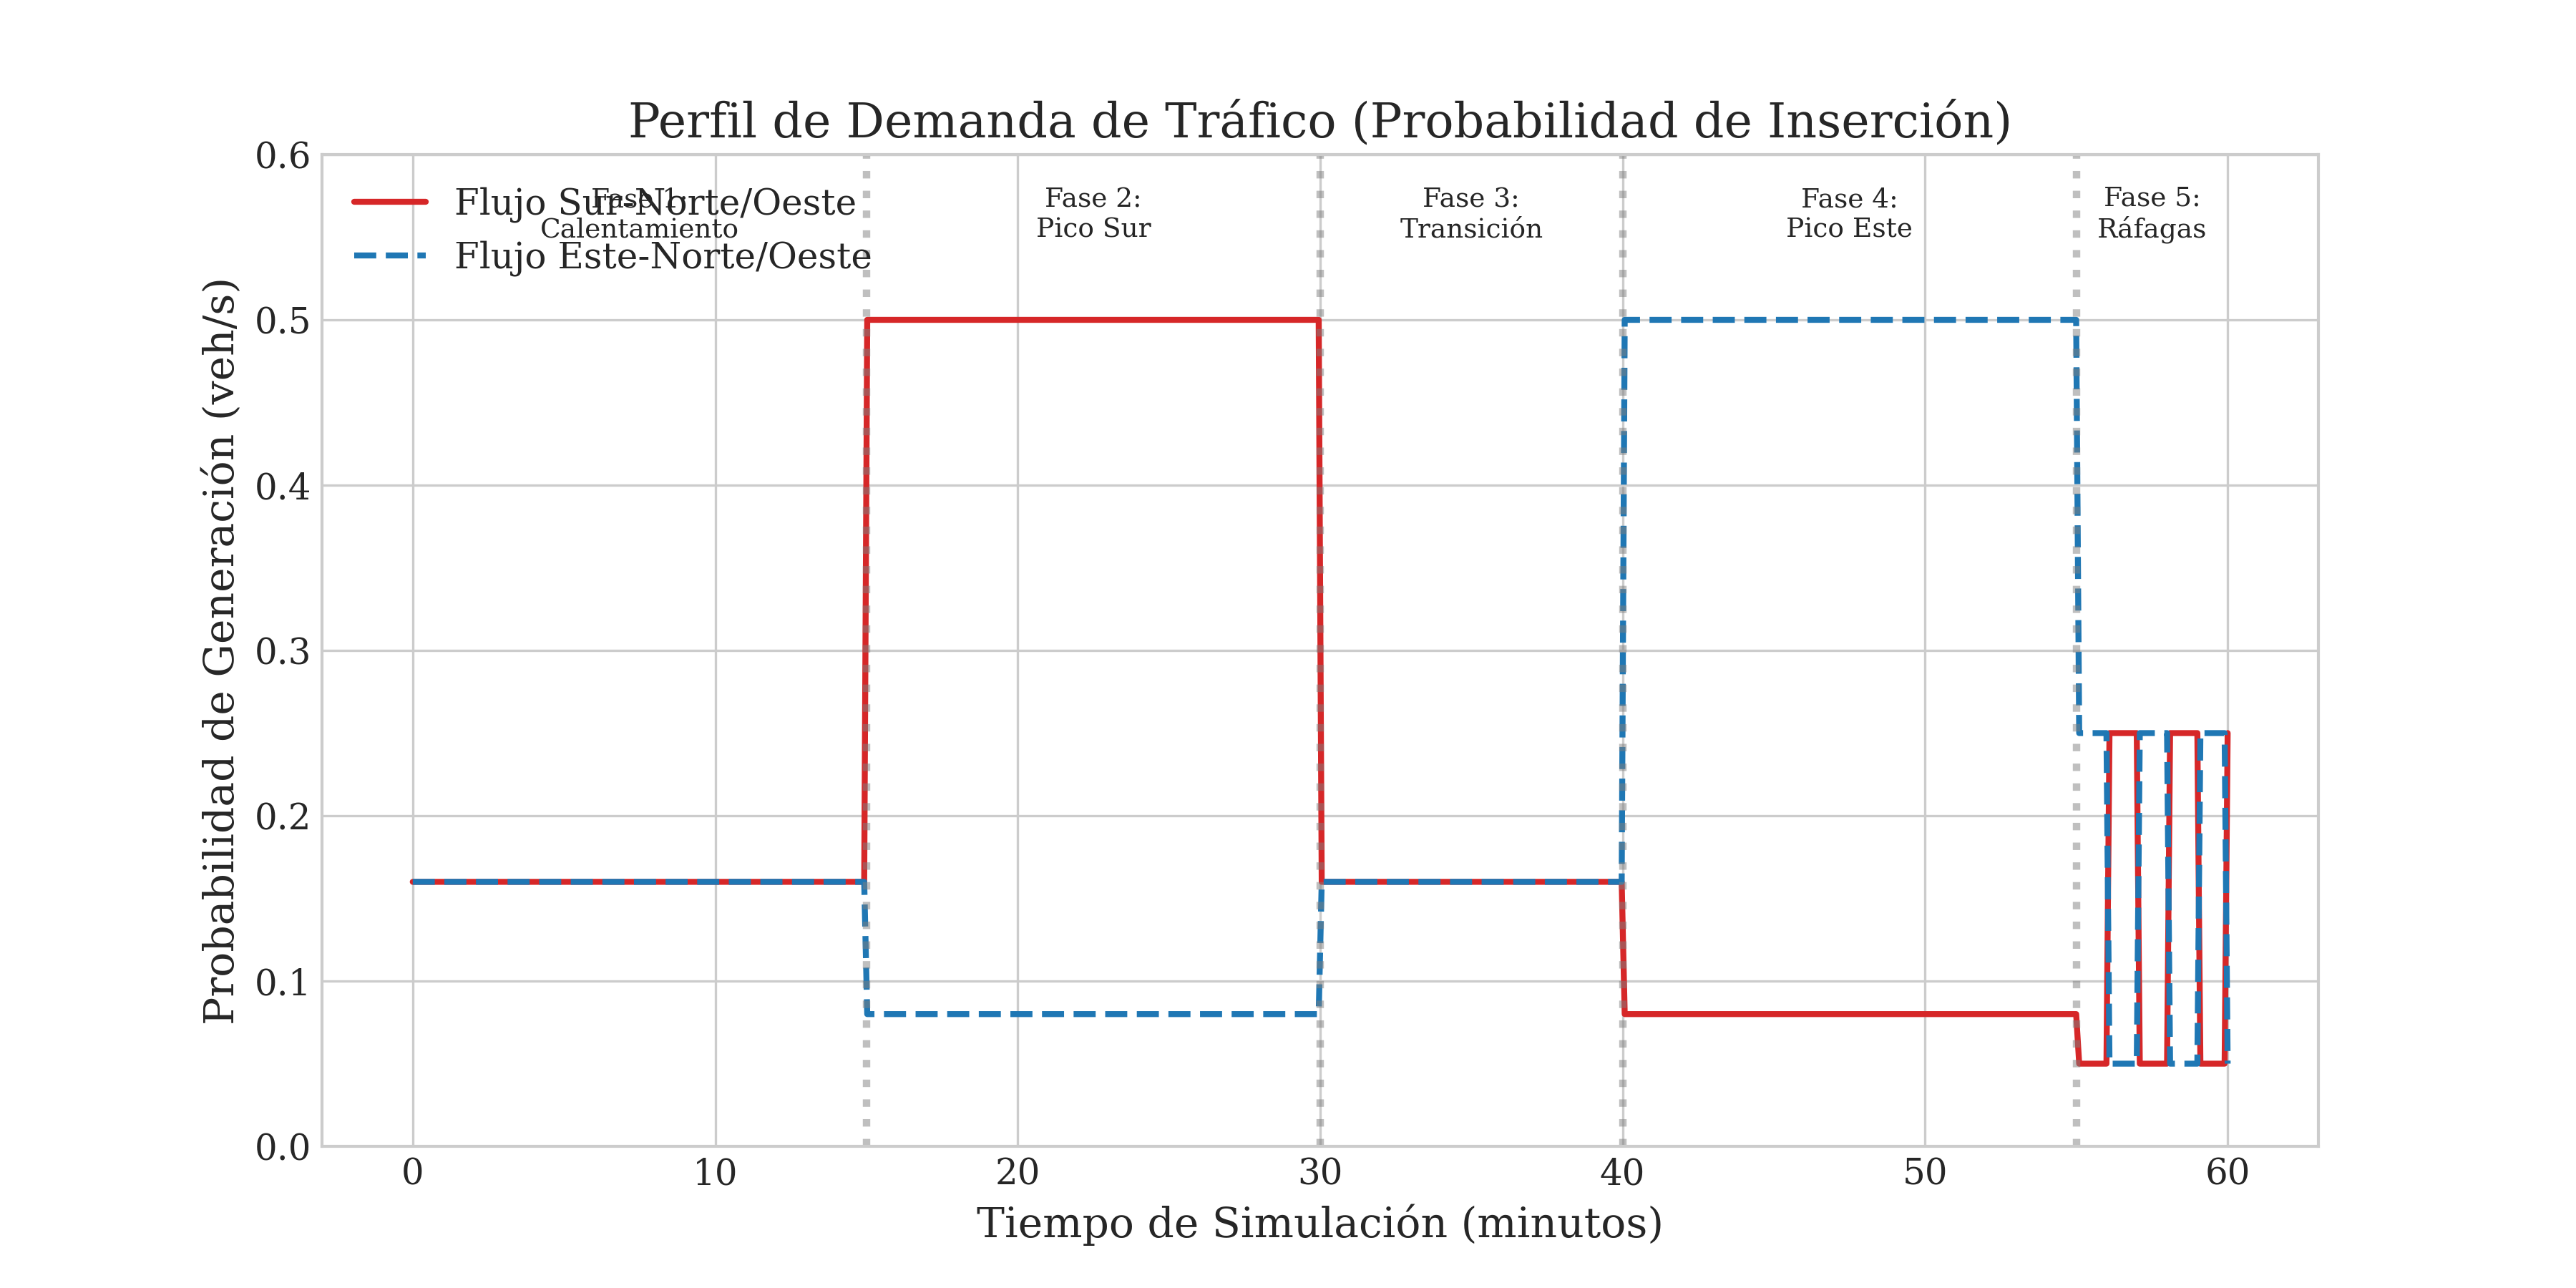
\includegraphics[width=0.8\textwidth]{images/traffic_profile.png}
    \caption{Perfil de probabilidad de inserción vehicular a lo largo de la hora simulada.}
    \label{fig:traffic_profile}
\end{figure}

\section{Formulación del entorno RL}
El problema de control se modeló como un MDP con las siguientes definiciones:

\textbf{Espacio de Observación ($S$):}
Un vector continuo normalizado que incluye:
\begin{itemize}
    \item Densidad de cola por carril ($d \in [0,1]$).
    \item Número de vehículos detenidos.
    \item Fase activa actual (one-hot encoding).
    \item Tiempo transcurrido desde el último cambio de fase.
\end{itemize}

\textbf{Espacio de Acciones ($A$):}
Un conjunto discreto binario:
\begin{itemize}
    \item $a=0$: Mantener la fase actual.
    \item $a=1$: Iniciar transición a la siguiente fase.
\end{itemize}
\textit{Restricción:} Se impone un tiempo de verde mínimo (\texttt{min\_green = 10s}) para evitar cambios oscilatorios que serían peligrosos en la práctica.

\textbf{Función de Recompensa ($R$):}
El diseño de la función de recompensa se fundamentó en un análisis iterativo de la literatura sobre control semafórico con DRL y en pruebas empíricas propias \cite{review_rasheed2020,presslight2019}. Inicialmente se consideró maximizar el \textit{throughput} directo, pero los experimentos mostraron que minimizar la longitud de cola resultaba en una política más eficiente y estable, permitiendo indirectamente un mayor flujo vehicular. Con base en ello, se formuló una función compuesta para balancear eficiencia y equidad:
\begin{equation}
    R_t = - w_{queue} \sum Q_t - w_{unbalance} |Q_{NS} - Q_{EO}| - w_{switch} \mathbb{I}_{change}
\end{equation}
Donde:
\begin{itemize}
    \item $R_t$: Recompensa total en el paso $t$.
    \item $Q_t$: Longitud de cola total.
    \item $|Q_{NS} - Q_{EO}|$: Diferencia absoluta de colas entre fases.
    \item $\mathbb{I}_{change}$: Indicador de cambio de fase.
    \item Pesos: $w_{queue}=1.0$, $w_{unbalance}=0.2$, $w_{switch}=5.0$.
\end{itemize}

\begin{figure}[H]
    \centering
    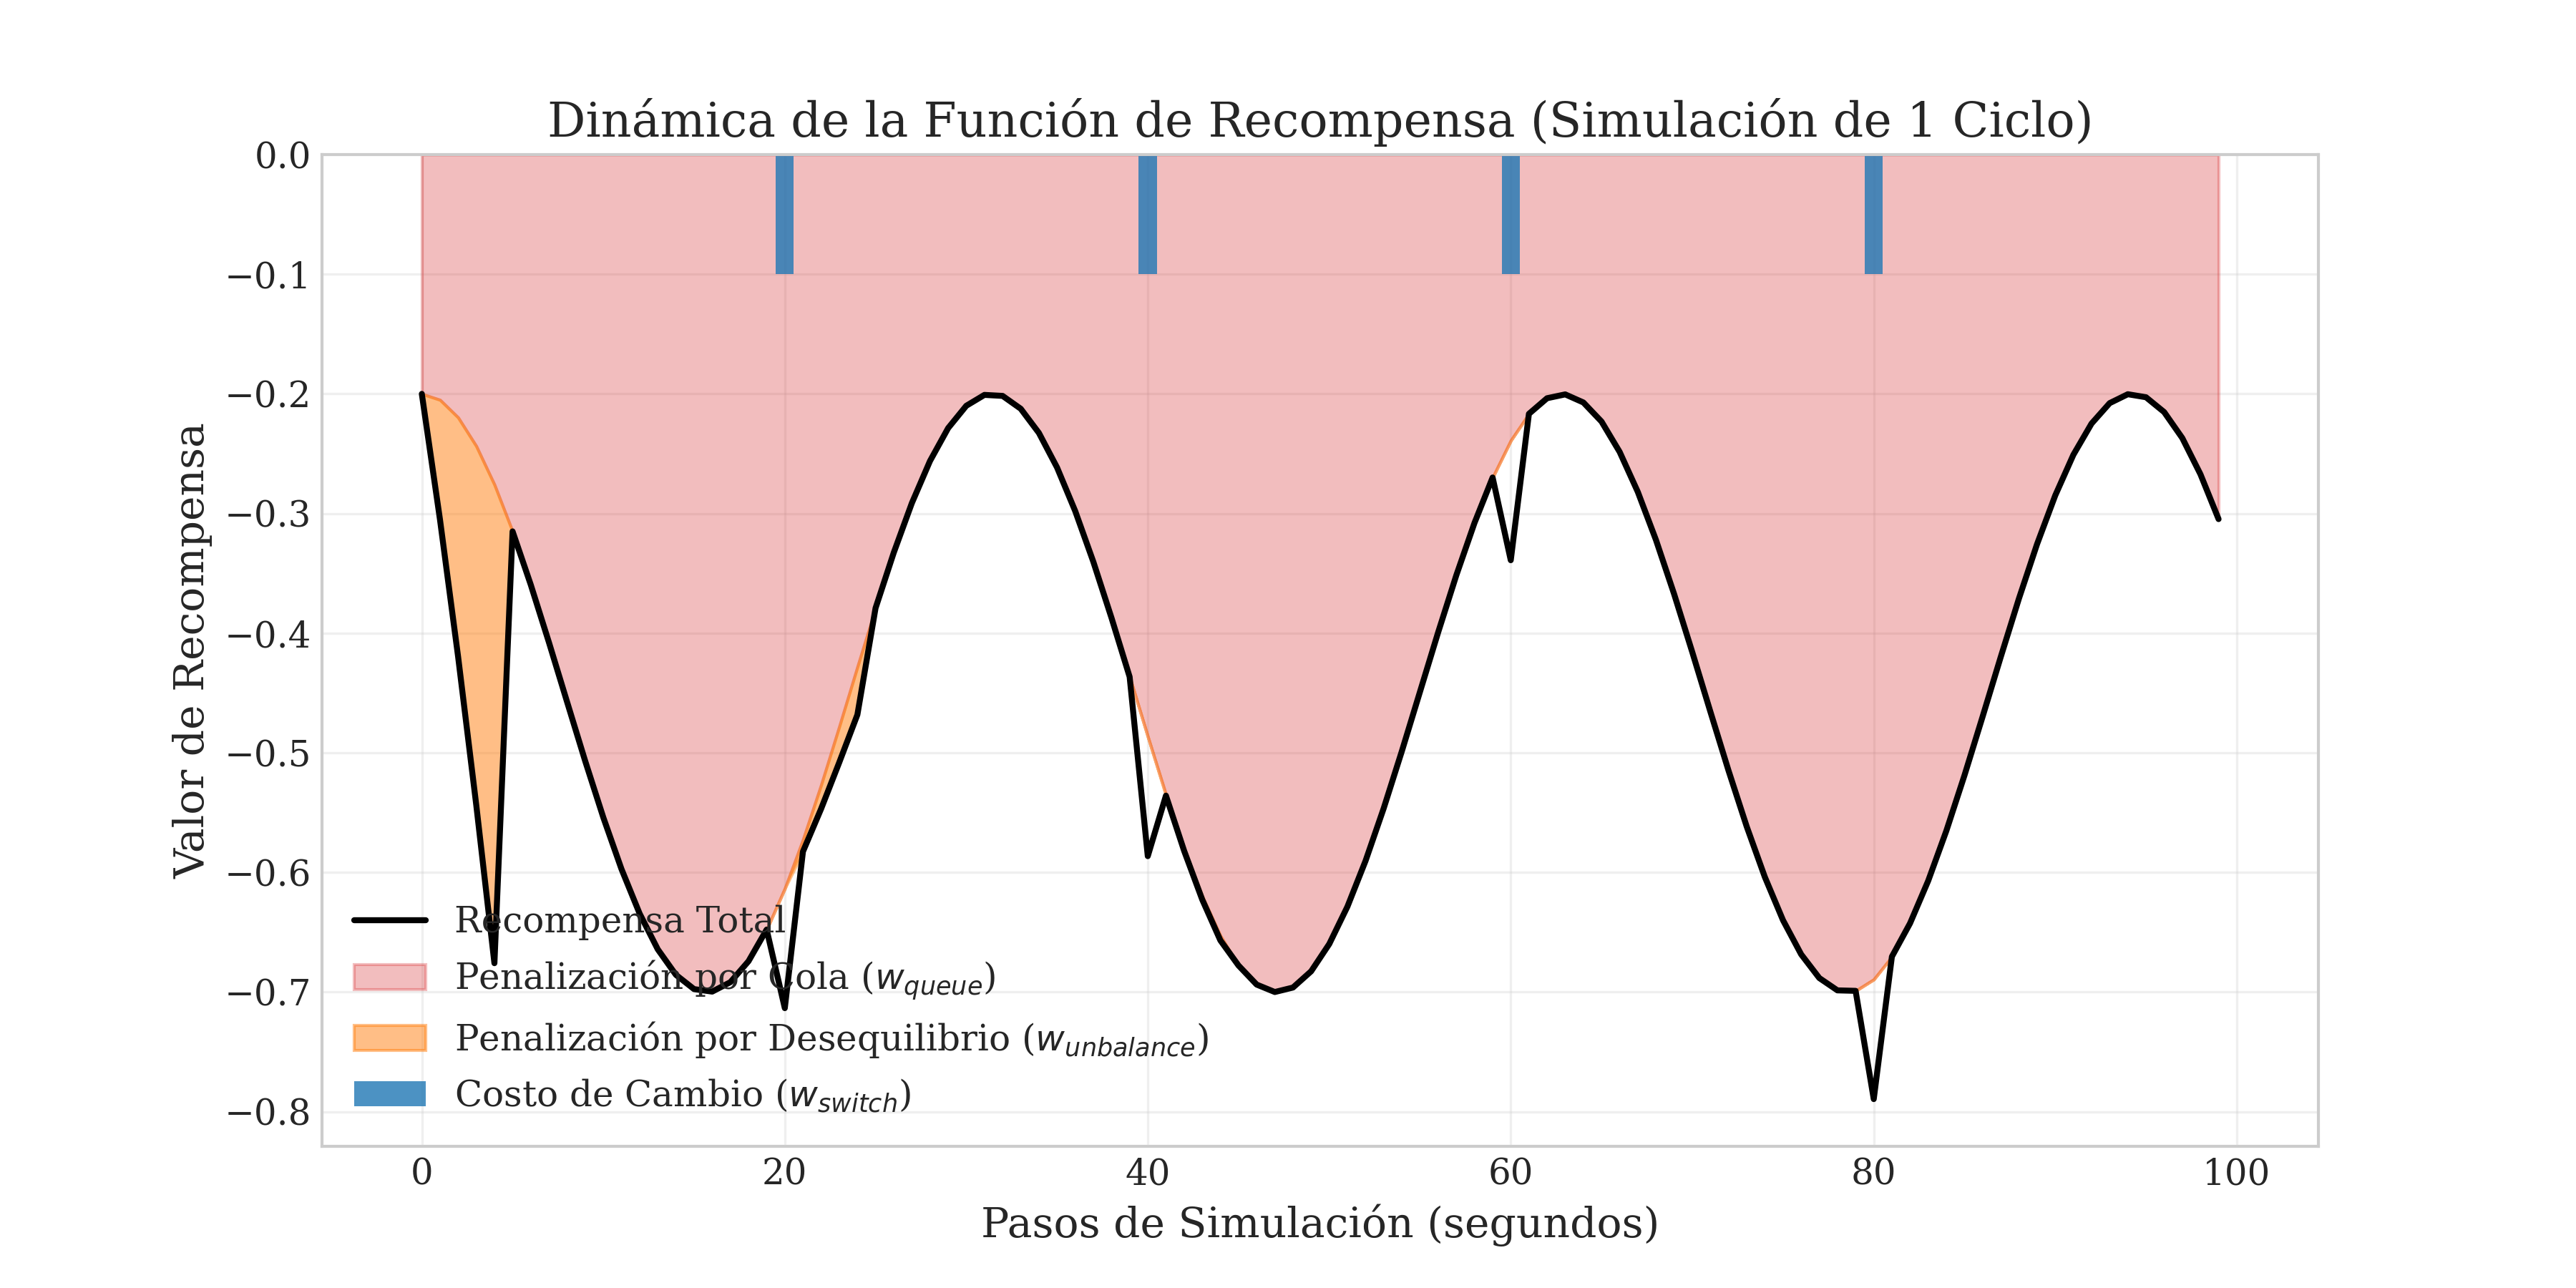
\includegraphics[width=0.8\textwidth]{images/reward_composition.png}
    \caption{Dinámica de la función de recompensa. Se observa cómo la penalización por cola domina, pero el desequilibrio crece si se ignora una fase.}
    \label{fig:reward_composition}
\end{figure}

Esta estructura incentiva al agente a vaciar las colas y, al mismo tiempo, lo penaliza si descuida una dirección o cambia de luz demasiado rápido.

\section{Arquitectura y configuración del algoritmo PPO}
Se utilizó la implementación de \textbf{Stable-Baselines3} \cite{stable_baselines3_2021} sobre un entorno estandarizado con \textbf{Gymnasium} \cite{gymnasium_2023}, empleando una arquitectura de red neuronal de dos capas ocultas de 64 neuronas cada una (MlpPolicy). Los hiperparámetros óptimos, encontrados mediante una búsqueda bayesiana con \textbf{Optuna} \cite{optuna_2019}, fueron:

\begin{table}[H]
    \centering
    \begin{tabular}{@{}lll@{}}
        \toprule
        \textbf{Hiperparámetro} & \textbf{Valor} & \textbf{Descripción} \\ \midrule
        \texttt{learning\_rate} & $3 \times 10^{-4}$ & Tasa de aprendizaje del optimizador Adam. \\
        \texttt{n\_steps} & 4096 & Pasos por actualización de política. \\
        \texttt{batch\_size} & 2048 & Tamaño del lote para el descenso de gradiente. \\
        \texttt{gamma} ($\gamma$) & 0.99 & Factor de descuento para recompensas futuras. \\
        \texttt{gae\_lambda} & 0.95 & Factor de suavizado para GAE. \\
        \texttt{clip\_range} & 0.2 & Rango de recorte para la función objetivo de PPO. \\
        \texttt{ent\_coef} & 0.01 & Coeficiente de entropía para fomentar exploración inicial. \\ \bottomrule
    \end{tabular}
    \caption{Hiperparámetros óptimos del agente PPO.}
    \label{tab:hyperparameters}
\end{table}

El entrenamiento se ejecutó durante \textbf{500,000 pasos de tiempo}, lo cual demostró ser suficiente para la convergencia de la política.

\section{Flujo de entrenamiento y simulación}
El proceso completo se desarrolló de la siguiente manera:
\begin{enumerate}
    \item Inicialización del entorno SUMO con tráfico dinámico.
    \item Ejecución del episodio durante 3600 pasos (equivalentes a 1 hora simulada).
    \item El agente observa el estado, determina una acción y la aplica mediante TraCI.
    \item SUMO avanza un paso de simulación y devuelve la recompensa correspondiente.
    \item PPO ajusta la política con base en los datos recolectados.
    \item Al finalizar el entrenamiento, el modelo se evalúa en 10 episodios independientes de 1 hora cada uno (N=10), comparándolo con un semáforo fijo de referencia para garantizar la validez estadística de los resultados.
\end{enumerate}

\begin{figure}[H]
    \centering
    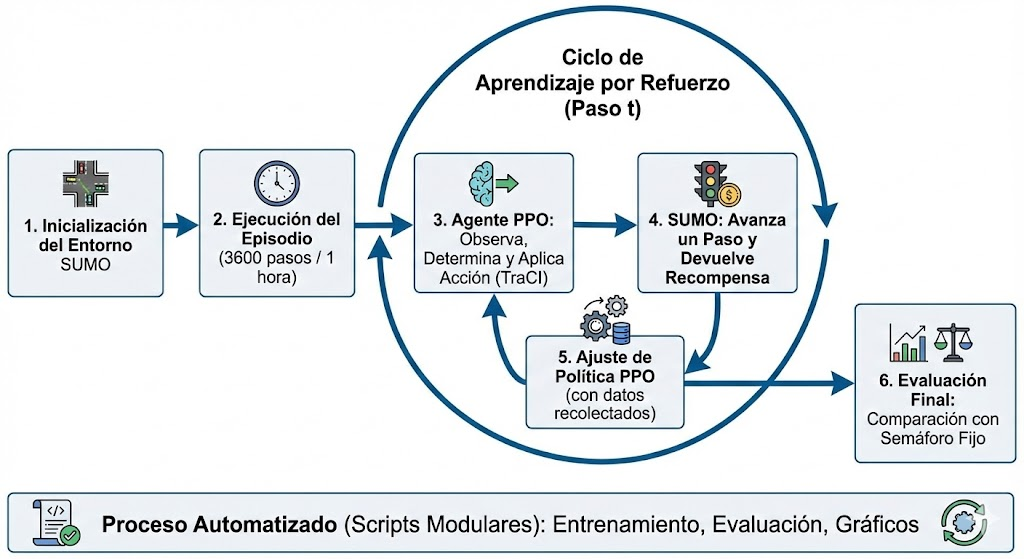
\includegraphics[width=0.8\textwidth]{images/flujo_entrenamiento.png}
    \caption{Diagrama de flujo del proceso de entrenamiento y simulación.}
    \label{fig:training_flow}
\end{figure}

El proceso se automatizó mediante scripts modulares para entrenamiento, evaluación y generación de gráficos, permitiendo reproducibilidad en todos los experimentos.
